\chapter{Théorèmes des travaux virtuels}
\section{Pour des déplacements infinitésimaux de corps indéformable}
	\subsection{Problème à résoudre}
	Avant toute chose, \textit{les théorèmes des travaux virtuels s'appliquent
	à des situations d'équilibre.} Dans un tel problème, nous avons des forces 
	de volume $f_i$, de surfaces associées à $\vec{n}$, $T_i^{(n)}$, des 
	déplacements résultant de ces deux forces mais aussi des contraintes 
	résultant de ces forces $\tau_{ij}$. Pour résoudre un tel système, on peut 
	utiliser :
	\begin{itemize}
	\item[$\bullet$] Équilibre en volume
		\begin{itemize}
		\item \textit{Translation} : $\tau_{ji,j}+f_i = 0$
		\item \textit{Rotation} : $\tau_{[ij]} =0\qquad\text{ou}\qquad \tau_{ij}=
		\tau_{ji}$
		\end{itemize}
	\item[$\bullet$] Équilibre en surface : $T_i^{(n)} = \tau_{ji}n_j$
	\item[$\bullet$] Les équations de comportement
	\item[$\bullet$] Les équations de compatibilité
	\end{itemize}

	\subsection{Pourquoi les théorèmes des travaux virtuels ?}
	Si l'on a toutes ces belles équations, pourquoi un nouveau théorèmes ? Les 
	raisons sont multiples : impossible de trouver des solutions analytiques, 
	application plus facile, formule indépendante du domaine d'application, 
	\dots
	
	\subsection{Grandeurs réelles et virtuelles}
	Deux définitions de grandeurs sont à énoncer 
	\begin{description}
	\item[Réelles] il s'agit des grandeurs (forces, déplacements, contraintes, 
	\dots) \textbf{réellement} appliquées au milieu ou subie par le milieu 
	continu étudié.
	\item[Virtuelles] il s'agit de grandeurs \textbf{arbitraires} choisies 
	judicieusement en fonction de ce que l'on veut calculer.
	\end{description}
	
	
	\subsection{Travail virtuel des forces extérieures}
	Nous allons considérer deux ensembles :
	\begin{enumerate}
	\item Virtuels : déplacement $u_i'$
	\item Réel : forces de volume et de surface : $f_i\ dV,\quad, T_i^{(n)}\ dS$
	\end{enumerate}
	On \textsc{définit} ($\equiv$) le travail virtuel des forces extérieures comme 
	le produit scalaire \textit{force*déplacement}
	\retenir{\begin{equation}
	T_{ext}' \equiv \int_V f_iu_i'\ dV + \oint_S T_i^{(n)}u_i'\ dS
	\end{equation}}\ 
	
	Le terme $f_iu_i'\ dV$ est le travail des forces de volume tandis que le second 
	terme est le travail des forces de surface, ou l'on considère toute la surface 
	fermée.


	\subsection{Calculs préliminaires}
	Nous allons restreindre les déplacements virtuels à des déplacements 
	\textbf{infinitésimaux} de corps \textbf{indéformable} 
	\begin{equation}
	\overline{u_P'} = \overline{u_Q'} + \overline{\theta'}\times\overline{QP}
	\end{equation}
	\begin{wrapfigure}[8]{r}{3.2cm}
	\vspace{-5mm}
	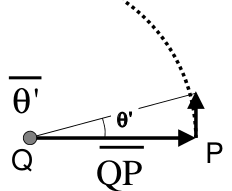
\includegraphics[scale=0.4]{ch8/image1.png}
	\captionof{figure}{ }
	\end{wrapfigure}
	Considérons le point $Q$ de référence. Le déplacement virtuel de $P$ est 
	une rotation de $\overline{OP}$ autour de $Q$ d'un angle $\theta$. Si 
	ce déplacement est infiniment petit, il s'agit de la tangente au cercle et 
	on peut l'exprimer à l'aide d'un produit vectoriel : si ce n'était pas le 
	cas, ce ne serait pas tangent et bye bye le produit vectoriel.\\
	
	Pourquoi est-ce si important d'avoir un produit vectoriel ? Car il est 
	nécessaire d'en avoir un pour exprimer la résultante de couple nulle. 
	Reprenons notre travail extérieur
	\begin{equation}
	T_{ext}' \equiv \int_V \overline{f}.\overline{u_P'}\ dV +\oint_S 
	\overline{T}^{(n)}.\overline{u_P'}\ dS
	\end{equation}
	En remplaçant $\overline{u_P'}$ par son expression
	\begin{equation}
	T_{ext}' \equiv \int_V \overline{f}.(\overline{u_Q'} + \overline{\theta'}
	\times\overline{QP})\ dV +\oint_S 	\overline{T}^{(n)}.(\overline{u_Q'} + 
	\overline{\theta'}\times\overline{QP})\ dS
	\end{equation}
	Comme $Q$ est un point fixe de référence ne dépendant pas de $x,y,z$, son 
	déplacement est une grandeur que l'on peut sortir de l'intégrale. De 
	même, $\vec  \theta'$ est une rotation : ne dépend pas des axes. Il faut 
	cependant faire une petite manipulation pour mettre $\vec \theta'$ en 
	évidence :
	\begin{equation}
	T_{ext}' \equiv \overline{u_Q'}\left[\int_V\overline{f}\ dV + \oint_S 
	\overline{T}^{(n)}\ dS\right] + \overline{\theta'}\left[\int_V (
	\overline{QP}\times\overline{f})\ dV + \oint_S(\overline{QP}\times
	\overline{T}^{(n)})\ dS\right]
	\end{equation}
	Les expressions de la résultante des forces et du moment résultant des 
	forces par rapport au point $Q$ apparaissent naturellement de sorte 
	que l'on puisse écrire
	\begin{equation}
	T_{ext}' \equiv\overline{u_Q'}.\overline{R}+\overline{\theta'}.\overline{
	C_Q}
	\end{equation}
	
	\subsection{Le théorème}
	Voici l'énoncé complet sous une forme systématique. "\textit{Je vous 
	invite à l'imprimer et à la coller sur le miroir de votre salle de bain.}"\ \\
	
	\theor{\textsc{Trav. virt. pour des dep. infinitésimaux de corps indéformable}\
	\begin{enumerate}
	\item A l'équilibre
	\item le travail virtuel des forces extérieures
	\item est nul
	\item pour tout déplacement \textbf{infinitésimal} de corps indéformable.
	\end{enumerate}	
	$$	T_{ext}' \equiv\overline{u_Q'}.\overline{R}+\overline{\theta'}.\overline{
	C_Q}$$}


	\subsection{Le théorème direct}
	Afin de ne pas confondre avec le théorème indirect, reformulons ce théorème 
	avec des \textit{Si\dots alors\dots}\\
	
	\textbf{Si} on est à l'équilibre \textbf{alors} le travail virtuel des forces 
	extérieures est nul pour tout déplacement virtuel \underline{infinitésimal} de 
	corps indéformable.\ 
	
	\retenir{\begin{center}
	équilibre $\Longrightarrow\qquad \overline{R}=\overline{0}\qquad$ et $\qquad 
	\overline{C_Q}=\overline{0}\qquad \Longrightarrow T_{ext}'=0$
	\end{center}}
	
	\subsection{Le théorème réciproque}
		\subsubsection{Énonce}
		\textbf{Si} le travail virtuel des forces extérieures est nul pour tout 
		déplacement virtuel \underline{infinitésimal} de corps indéformable 
		\textbf{alors} on est à l'équilibre\footnote{C'est souvent le $\forall$ 
		qui est oublié, attention !}.
		$$T_{ext}' = 0\Longrightarrow\qquad \overline{u_Q'}.\overline{R}+
		\overline{\theta'}.\overline{C_Q}=0\qquad \forall \overline{u_Q'}, 
		\quad\overline{\theta'}$$
		
		\subsubsection{Démonstration}
		Comme ceci est valable $\forall\dots$, nous allons gentillement choisir.
		\begin{proof}\ 
		\begin{itemize}
		\item[$\bullet$] Choisissons une translation virtuelle quelconque
		$$\overline{u_Q'}.\overline{R}+\overline{\theta'}.\overline{C_Q}=0,\quad 
		\overline{\theta'}=\vec0\qquad\Longrightarrow \overline{R}=\overline{0}$$
		\item[$\bullet$] Choisissons une rotation virtuelle quelconque
		$$\overline{u_Q'}.\overline{R}+\overline{\theta'}.\overline{C_Q}=0,\quad 
		\overline{u_Q'}=\vec0\qquad\Longrightarrow \overline{C_Q}=\overline{0}$$		
		\end{itemize}
		\end{proof}
		

\section{Pour des déplacements quelconques}
	\subsection{Travail virtuel des forces intérieures}
	Reconsidérons nos deux ensembles, mais en plus supposons que l'équilibre soit 
	satisfait en surface :
	\begin{equation}
	T_i^{(n)} = \tau_{ji}n_j
	\end{equation}
	\danger On ne peut supposer la symétrie de $\tau_{ij}$ dès le départ, mais 
	ce résultat découlera du théorème.
	
	\subsection{Calculs préliminaires}
	Partons de la définition du travail extérieur et appliquons le théorème de 
	Gauss :
	\begin{equation}
	\oint_S T_i^{(n)}u_i'\ dS = \oint_S \tau_{ji}n_ju_i'\ dS = \int_V \partial_j
	(\tau_{ji}u_i')\ dV
	\end{equation}
	En appliquant la règle de dérivée d'un produit et le développement en une 
	partie symétrique/asymétrique :
	\begin{equation}
	\partial_j(\tau_{ji}u_i') = \tau_{ji,j}u_i'+\tau_{ji}u_{i,j}' = \tau_{ji,j}
	u_i' + \tau_{ji}u_{(i,j)}'+\tau_{ji}u_{[i,j]}'
	\end{equation}
	Notons (ceci est une \textbf{définition} !)
	\begin{equation}
	a_{ij}' \equiv u_{(i,j)}' \equiv \dfrac{1}{2}(u_{i,j}'+u_{j,i}')
	\end{equation}
	Le travail extérieur peut alors s'écrire
	\begin{equation}
	T_{ext}' = \int_v fiu_i'\ dV + \int_V [\tau_{ji,j}u_i'+\tau_{ji}a_{ij}'+
	\tau_{ji}u_{[i,j]}]\ dV
	\end{equation}
	En ordonnant les termes :
	\begin{equation}
	T_{ext}' \equiv \int_V(\tau_{ji,j}+f_i)u_i'\ dV + \int_V\tau_{ji}u_{[i,j]}'\ 
	dV + \int_V\tau_{ji}a_{ij}'\ dV
	\end{equation}
	S'il y a équilibre, les deux premiers termes sont nuls : équilibre de 
	translation en volume et équilibre de rotation en volume. Donc, à 
	l'équilibre, il reste pour des déplacements virtuels quelconques 
	\begin{equation}
	T_{ext}' = \int_V \tau_{ji}a_{ij}'\ dV
	\end{equation}
	Cette notion conduit à \textbf{définir} un travail virtuel pour les forces 
	intérieurs :
	\begin{equation}
	T_{int}' = -\int_V\tau_{ji}a_{ij}'\ dV
	\end{equation}
	Pourquoi ce signe? Juste pour avoir $T_{ext}'=-T_{int}$ (convention dans le 
	cadre de ce cours). A l'équilibre, le travail virtuel total sera donc 
	forcément nul
	\begin{equation}
	T_{tot}' \equiv  T_{ext}'+T_{int}'
	\end{equation}
	Comme $a_{ij}'$ est symétrique (def.) on peut écrire $T_{int}'$ de la sorte 
	(permutation des indices) :
	\begin{equation}
	T_{int}' = -\int_V\tau_{ji}a_{ji}'\ dV
	\end{equation}
	Ce qui donne, après avoir renommer les indices
	\begin{equation}
	T_{int}' = -\int_V\tau_{ij}a_{ij}'\ dV
	\end{equation}
	
	\subsection{Travail virtuel total}
	Reprenons la définition du travail virtuel total
	\begin{equation}
	T_{tot}' \equiv \int_V f_iu_i'\ dV + \oint_S T_i^{(n)}u_i'\ dS - \int_V 
	\tau_{ji}a_{ij}\ dV
\end{equation}		
	Et transformons la dernière intégrale (sachant que la partie symétrique 
	correspond à "tout" - la partie symétrique)
	\begin{equation}
	\begin{array}{ll}
	\tau_{ji}a_{ij}' &= \tau_{ji}u_{(i,j)}'\\
	&= \tau_{ji}u_{i,j}' - \tau_{ji}u_{[i,j]}'\\
	&= \partial_j(\tau_{ji}u_i')-\tau_{ji,j}u_i'-\tau_{ji}u_{[i,j]}'
	\end{array}
	\end{equation}
	En appliquant Gauss de façon inversée :\\
	\retenir{
	\begin{equation}
	T_{tot}' \equiv \int_V(\tau_{ji,j}+f_i)u_i'\ dV +\oint_S (T_i^{(n)}-\tau_{ji}
	n_j)u_i'\ dS + \int_V \tau_{ji}u_{[i,j]}'\ dV
	\end{equation}}
	
	\subsection{Le théorème}
	Il s'agit maintenant du théorème des travaux virtuels pour des déplacements 
	\textbf{quelconques} !\
	
	\theor{\textsc{Trav. virt. pour des des. quelconque}\ 
	\begin{enumerate}
	\item A l'équilibre
	\item le travail virtuel total
	\item est nul
	\item pour tout déplacement virtuel
	\end{enumerate}
	$$	T_{tot}' \equiv \int_V(\tau_{ji,j}+f_i)u_i'\ dV +\oint_S (T_i^{(n)}-\tau_{ji}
	n_j)u_i'\ dS + \int_V \tau_{ji}u_{[i,j]}'\ dV$$}
	
	\subsection{Le théorème direct}
	Reformulons notre beau théorème\\
	\textbf{Si} on est à l'équilibre, \textbf{alors} le travail virtuel total 
	est nul pour tout déplacement virtuel.
	\begin{center}
	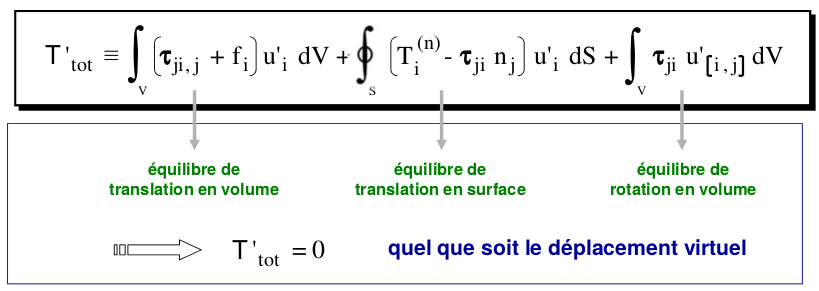
\includegraphics[scale=0.4]{ch8/image2}
	\captionof{figure}{ }
	\end{center}
		
		
	\subsection{Le théorème réciproque}
	\textbf{Si} le travail virtuel total est nul pour tout déplacement virtuel, 
	\textbf{alors} on est à l'équilibre.
	\begin{equation}
	T_{tot}' = 0\Longrightarrow\qquad 
	\int_V(\tau_{ji,j}+f_i)u_i'\ dV +\oint_S (T_i^{(n)}-\tau_{ji}
	n_j)u_i'\ dS + \int_V \tau_{ji}u_{[i,j]}'\ dV=0\qquad \forall u_i'
	\end{equation}
	Démontrons ce théorème des travaux virtuels pour des déplacements quelconques.
	On peut bien "choisir" car ceci est valable $\forall u_i'$.\\
	\begin{proof}\ \\
	\textsc{A.} 
	Nous allons faire trois choix de déplacement pour prouver notre théorème. 
	Commençons par considérer une translation virtuelle nulle partout en volume 
	et en surface, sauf sur une petite portion de \textbf{volume} ou elle est constante. 
	Les deux derniers termes de $T_{tot}'$ sont nuls. Comme je peux faire "balader" 
	cette portion de \textbf{volume}, j'ai toujours
	\begin{equation}
	(\tau_{ji,j}+f_i) = 0
	\end{equation}
	La première intégrale de $T_{tot}'$ est forcément nulle.\\
	
	\textsc{B.} 
	Maintenant, considérerons une translation virtuelle nulle partout en volume 
	et en surface, sauf sur une petite portion de \textbf{surface} ou elle est constante. 
	Comme je peux faire "balader" cette portion de \textbf{surface}, j'ai toujours
	\begin{equation}
	T_i^{(n)} = \tau_{ji}n_j
	\end{equation}
	L'intégrale rendue nulle par \textsc{A} est toujours valable, car nous venons 
	de faire un choix "virtuel", n’influençant pas sur notre choix réel. La seconde 
	intégrale de $T_{tot}'$ est forcément nulle (et la première, par \textsc{A}, 
	également).\\
	
	\textsc{C.} 
	Choisissons un déplacement nul partout en volume et en surface, sauf sur une 
	petite portion de \textbf{volume} où on le choisit quelconques. En faisant 
	également "balader" cette portion de volume\footnote{Les deux premières 
	intégrales étant nulles, celle-ci doit forcément l'être également.}
	\begin{equation}
	\tau_{ji}u'_{[i,j]} = 0
	\end{equation}
	où $\tau_{ji}$ est symétrique.
	\end{proof}



\section{Remarques}
	\subsection{Domaines de validité des théorèmes}
	Pour un déplacement de corps \textbf{indéformable}, les déplacements doivent 
	être infinitésimaux pour pouvoir exprimer les rotations à l'aide d'un produit 
	vectoriel. Les déplacements de corps indéformable $\equiv$ corps rigides 
	doivent ainsi toujours être infinitésimaux sinon le déplacement serait réel.\\
	
	Néanmoins, pour un déplacement \textbf{quelconque}, ceux-ci ne doivent 
	\textbf{pas} être infinitésimaux. \\
	
	Les déplacement virtuels :
	\begin{itemize}
	\item[$\bullet$] sont choisis en fonction de ce que l'on veut calculer
	\item[$\bullet$] ne doivent pas respecter les liaisons (forcément, si on veut 
	les calculer il vaut mieux les faire travailler)
	\end{itemize}
	
	\danger La loi de comportement n'intervient \textbf{pas} dans les théorèmes, 
	ils ne sont donc pas limités au cas du solide linéaire élastique.
	
	\subsection{Questions d'oral}
	\begin{itemize}
	\item[$\bullet$] \textit{Est-il nécessaire de prendre des déplacements 
	infinitésimaux}. \\
	La réponse de l'étudiant est souvent en quatre temps :
	\begin{enumerate}
	\item Long silence
	\item Regard effrayé, le silence se poursuit
	\item Il répond "Oui oui" pour me faire plaisir
	\item Non non
	\end{enumerate}
	La réponse est bien sûr non, tout comme la réponse à la prochaine question.
	\item[$\bullet$] \textit{Les déplacements virtuels doivent-ils respecter les 
	réactions de liaisons ?}
	\end{itemize}
